% !TeX spellcheck = en_US
\documentclass[12pt,fleqn]{article}


\usepackage[english]{babel}
\usepackage{amsmath}

\usepackage{texfiles/SpeedyGonzales}
\usepackage{texfiles/MediocreMike}
\usepackage{multicol}
\usepackage{subcaption}


\title{\vspace*{-3.75cm}Classifying a Contry's COVID-19 Fatalities}
\author{Søren Holm, Oskar Wiese, Anders Henriksen and Anne Pedersen \\
	\small {\texttt{\{s183911,s183917,s183904,s174300\}@student.dtu.dk}}}
\date{\today}


\pagestyle{fancy}
\fancyhf{}
\lhead{Title}
\rfoot{Page \thepage{} of \pageref{LastPage}}
\graphicspath{{imgs/}}

\begin{document}
	
	\maketitle
	 
	
	\begin{abstract} %TODO: Write section
		
	\end{abstract}
	
	\begin{multicols}{2}
		
		
		\section{Introduction} %TODO: Add something about GP
		The novel corona virus COVID-19 has affected the lives of billions of people all around the world. This project has collected a dataset of different measures for each country and then uses uncertainty sampling to classify countries by the number of COVID-19 related fatalities. Lastly we compare different ways of sampling to find the one that gets a satisfying accuracy the fastest. Our initial hypothesis is that margin sampling performs better than the other samplers due to the relatively small amount of classes. 
		
		\section{Data}
		The dataset was constructed from several different datasets \cite{density, corona, alder, bnp, region, healthcare, turist}. For each country in the world with at least one COVID-19 related fatality, we collected eight features; the country's GDP per capita, population density per km$^2$, continent, median age of the population, index of quality of healthcare system, number of tourists per year in thousands, and the population count. These features were used to classify the countries by number of fatalities in three classes. 60 \% of the data was used for training, while the remaining 40 \% was used for testing. %TODO: define classes

		\section{Methods}
		\texttt{Code available at \url{github.com/sorenmulli/active_learning_cases}} \newline
		A gaussian process classifier has been implemented to predict on the training set, using uncertainty sampling for pool-based sampling.

		Pool-based sampling is a cycle of the learner getting a labeled dataset, training the model and then evaluating on an unlabeled test set. The labels subset of the unlabeled pool that the learner was most uncertain about are then queried and the samples are added to the training set. Then the cycle repeats until the model reaches a satisfying level of accuracy.  
		
		For the uncertainty sampling, least confident, margin sampling, entropy and random sampling have been used as uncertainty measures.
		
		\begin{itemize}
			\item \textbf{Least confident} samples the datapoints from the pool with the lowest probability for their most likely label.
			\item \textbf{Margin} sampling samples the points with the smallest difference between the two most likely labels.
			\item \textbf{Entropy} samples the points which have the maximum negative value over the likelyhood of the label times the log of the likelyhood of the label, summed over each label.
			\item \textbf{Random Sampling} samples datapoints randomly from the pool.
		\end{itemize}
		 
		The project aims to compare the performance of least confident, margin sampling and entropy on the proposed classification problem. 
		 
	\end{multicols}		

	\section{Results} %TODO: Write section
			\begin{figure}[H]
			\centering
			\begin{minipage}{.5\textwidth}
				\centering
				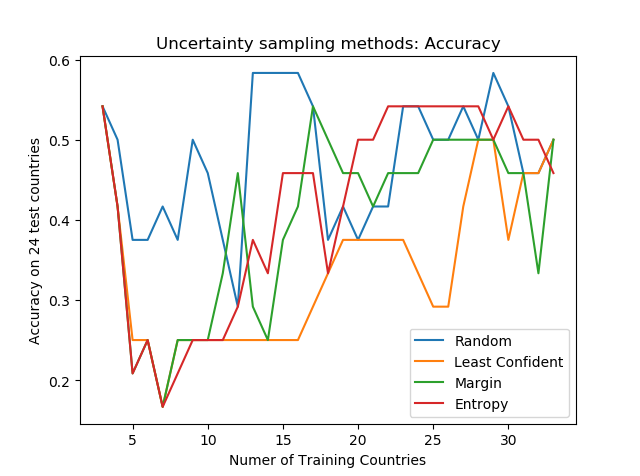
\includegraphics[width=\linewidth]{../src/saved_data/Accuracies}
				\caption{The accuracies of all four uncertainty sampling methods for every iteration.}
				\label{fig:accuracies}
			\end{minipage}%
			\begin{minipage}{.5\textwidth}
				\centering
				\includegraphics[width=\linewidth]{"../src/saved_data/Class balancing"}
				\caption{The proportion of the largest class in the pool at each iteration. Balance is at 0.33}
				\label{fig:class-balancing}
			\end{minipage}
			\end{figure}
			
		
	\begin{multicols}{2}

		\section{Discussion} %TODO: Write section
			
		% 	
		As seen from figure \ref{fig:accuracies}, the three uncertainty sampling methods all seem intertwined. Furthermore, it looks like the random sampling outperforms the proposed methods which will be discussed later. The data that has been collected  in this project does not portray the real data that describes the number of COVID-19 fatalities in a country. Many other variables that are far more complex than simple numbers can impact the infection curve. Thus, the uncertainty sampling methods may seem no better than random. Moreover, if there are many outliers in the data-set that have no co-linearity, then the constructed model will not benefit by being trained on these data-points. \noindent
		
		Another important factor is the class imbalance, see figure \ref{fig:class-balancing}. The reason why all of the experiments starts with a fairly high accuracy is due to the fact that classes are balanced (the model starts with a country from each class ). As the number of training countries increases the uncertainty methods proposed in this project, will start filling up a whole class before starting to sample from other classes. This creates an imbalanced data-set which in turn makes the accuracy of the model very poor. 
			
			
		\section{Learning outcome} %TODO: Write section
		Throughout the process of conducting the experiment and writing the report, a deeper understanding of the implementation and inner workings of active learning and uncertainty sampling and has been achieved. The unintuitive result of random sampling being close to on par with other methods has shown to not generally be the case but is rather caused by the class imbalance created when sampling from the pool. Realizing this allows for counteractive measures to be taken in the future to uphold this balance. Other minutia like increasing number of optimizer restarts and using an appropriate kernel have also proved to play an important role for sensible results.
			
	\end{multicols}

\newpage
	\begin{thebibliography}{9}
	
	
		
		\bibitem{density} Wikipedia contributors: "List of countries and dependencies by population density", Date of last revision: 22 March 2020 15:25 UTC. Visited at,  \url{ https://en.wikipedia.org/w/index.php?title=List_of_countries_and_dependencies_by_population_density&oldid=946809073}
		
		\bibitem{corona} Balaaje from Kaggle: "Coronavirus (COVID-19) dataset" with data from \url{https://www.worldometers.info/coronavirus/}. Visited at, \url{https://www.kaggle.com/balaaje/coronavirus-covid19-dataset}
		
		\bibitem{alder} World Population Review: "Countries by Median Age 2018". Visited at, \url{https://worldpopulationreview.com/countries/median-age/}
		
		\bibitem{bnp} International Monetary Fund: "GDP per capita, current prices", ©IMF, 2019. Visited at, \url{https://www.imf.org/external/datamapper/NGDPDPC@WEO/OEMDC/ADVEC/WEOWORLD}
		
		\bibitem{region} J. SnowLabs, Datahub.io: "Country and Continent Codes List" . Can be found at, \url{https://datahub.io/JohnSnowLabs/country-and-continent-codes-list}
		
		\bibitem{healthcare} Numbeo.com: "Health Care Index by Country 2020". Visited at, \url{https://www.numbeo.com/health-care/rankings_by_country.jsp}
		
		\bibitem{turist} World Economic Forum: "Travel and Tourism Competitiveness Index", © 2020 World Economic Forum. Visited at, \url{http://reports.weforum.org/travel-and-tourism-competitiveness-report-2019/rankings/}
		
		
		
		
		
	\end{thebibliography}
	
	%\section{Appendix}
	
	
\end{document}

















